\documentclass{standalone}
\usepackage{tikz}
\usetikzlibrary{patterns, positioning}

\begin{document}
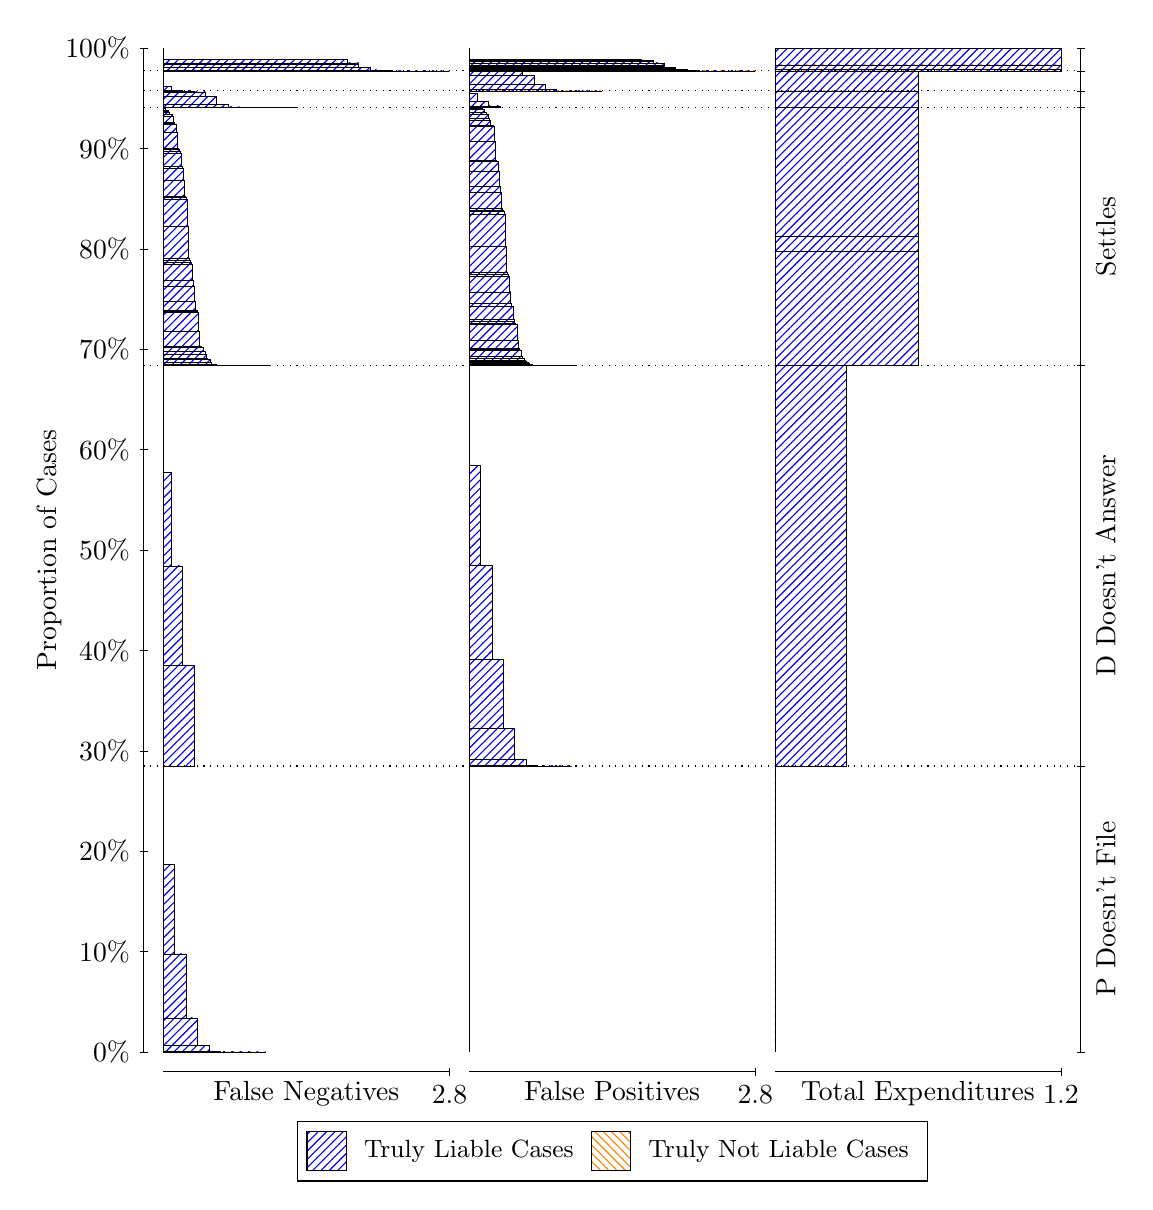
\begin{tikzpicture}
\draw[black, very thin] (1.5,1.75) -- (1.5,14.5);
\node[rotate=90, anchor=center] at (0.3, 8.125) {Proportion of Cases};
\draw[black, very thin] (1.45,1.75) -- (1.55,1.75);
\node[anchor=east] at (1.45, 1.75) {0\%};
\draw[black, very thin] (1.45,3.025) -- (1.55,3.025);
\node[anchor=east] at (1.45, 3.025) {10\%};
\draw[black, very thin] (1.45,4.3) -- (1.55,4.3);
\node[anchor=east] at (1.45, 4.3) {20\%};
\draw[black, very thin] (1.45,5.575) -- (1.55,5.575);
\node[anchor=east] at (1.45, 5.575) {30\%};
\draw[black, very thin] (1.45,6.85) -- (1.55,6.85);
\node[anchor=east] at (1.45, 6.85) {40\%};
\draw[black, very thin] (1.45,8.125) -- (1.55,8.125);
\node[anchor=east] at (1.45, 8.125) {50\%};
\draw[black, very thin] (1.45,9.4) -- (1.55,9.4);
\node[anchor=east] at (1.45, 9.4) {60\%};
\draw[black, very thin] (1.45,10.675) -- (1.55,10.675);
\node[anchor=east] at (1.45, 10.675) {70\%};
\draw[black, very thin] (1.45,11.95) -- (1.55,11.95);
\node[anchor=east] at (1.45, 11.95) {80\%};
\draw[black, very thin] (1.45,13.225) -- (1.55,13.225);
\node[anchor=east] at (1.45, 13.225) {90\%};
\draw[black, very thin] (1.45,14.5) -- (1.55,14.5);
\node[anchor=east] at (1.45, 14.5) {100\%};

\draw[black, very thin] (13.4,1.75) -- (13.4,14.5);
\draw[black, very thin] (13.35,1.75) -- (13.45,1.75);
\node[anchor=west] at (13.35, 1.75) {};
\draw[black, very thin] (13.35,5.382) -- (13.45,5.382);
\node[anchor=west] at (13.35, 5.382) {};
\draw[black, very thin] (13.35,10.471) -- (13.45,10.471);
\node[anchor=west] at (13.35, 10.471) {};
\draw[black, very thin] (13.35,13.75) -- (13.45,13.75);
\node[anchor=west] at (13.35, 13.75) {};
\draw[black, very thin] (13.35,13.956) -- (13.45,13.956);
\node[anchor=west] at (13.35, 13.956) {};
\draw[black, very thin] (13.35,14.211) -- (13.45,14.211);
\node[anchor=west] at (13.35, 14.211) {};
\draw[black, very thin] (13.35,14.5) -- (13.45,14.5);
\node[anchor=west] at (13.35, 14.5) {};

\draw[black, very thin, pattern color=blue, pattern=north east lines] (1.75,1.75) rectangle (3.0476,1.75);
\draw[black, very thin, pattern color=blue, pattern=north east lines] (1.75,1.75) rectangle (2.9034,1.75);
\draw[black, very thin, pattern color=blue, pattern=north east lines] (1.75,1.75) rectangle (2.7593,1.75);
\draw[black, very thin, pattern color=blue, pattern=north east lines] (1.75,1.75) rectangle (2.6151,1.7503);
\draw[black, very thin, pattern color=blue, pattern=north east lines] (1.75,1.7503) rectangle (2.4709,1.7572);
\draw[black, very thin, pattern color=blue, pattern=north east lines] (1.75,1.7572) rectangle (2.3267,1.8318);
\draw[black, very thin, pattern color=blue, pattern=north east lines] (1.75,1.8318) rectangle (2.1825,2.1829);
\draw[black, very thin, pattern color=blue, pattern=north east lines] (1.75,2.1829) rectangle (2.0384,2.995);
\draw[black, very thin, pattern color=blue, pattern=north east lines] (1.75,2.995) rectangle (1.8942,4.1337);
\draw[black, very thin, pattern color=orange, pattern=north west lines] (1.75,4.1337) rectangle (1.75,4.1337);
\draw[black, very thin, pattern color=blue, pattern=north east lines] (1.75,4.1337) rectangle (1.75,5.382);
\draw[black, very thin, pattern color=blue, pattern=north east lines] (1.75,5.382) rectangle (2.1393,6.6566);
\draw[black, very thin, pattern color=blue, pattern=north east lines] (1.75,6.6566) rectangle (1.9951,7.9231);
\draw[black, very thin, pattern color=blue, pattern=north east lines] (1.75,7.9231) rectangle (1.8509,9.1124);
\draw[black, very thin, pattern color=orange, pattern=north west lines] (1.75,9.1124) rectangle (1.75,9.1124);
\draw[black, very thin, pattern color=blue, pattern=north east lines] (1.75,9.1124) rectangle (1.75,10.471);
\draw[black, very thin, pattern color=blue, pattern=north east lines] (1.75,10.471) rectangle (3.1125,10.471);
\draw[black, very thin, pattern color=blue, pattern=north east lines] (1.75,10.471) rectangle (3.0476,10.471);
\draw[black, very thin, pattern color=blue, pattern=north east lines] (1.75,10.471) rectangle (2.9827,10.471);
\draw[black, very thin, pattern color=blue, pattern=north east lines] (1.75,10.471) rectangle (2.9683,10.471);
\draw[black, very thin, pattern color=blue, pattern=north east lines] (1.75,10.471) rectangle (2.9179,10.471);
\draw[black, very thin, pattern color=blue, pattern=north east lines] (1.75,10.471) rectangle (2.9034,10.471);
\draw[black, very thin, pattern color=blue, pattern=north east lines] (1.75,10.471) rectangle (2.853,10.471);
\draw[black, very thin, pattern color=blue, pattern=north east lines] (1.75,10.471) rectangle (2.8386,10.471);
\draw[black, very thin, pattern color=blue, pattern=north east lines] (1.75,10.471) rectangle (2.8241,10.471);
\draw[black, very thin, pattern color=blue, pattern=north east lines] (1.75,10.471) rectangle (2.7881,10.471);
\draw[black, very thin, pattern color=blue, pattern=north east lines] (1.75,10.471) rectangle (2.7737,10.471);
\draw[black, very thin, pattern color=blue, pattern=north east lines] (1.75,10.471) rectangle (2.7593,10.471);
\draw[black, very thin, pattern color=blue, pattern=north east lines] (1.75,10.471) rectangle (2.7232,10.471);
\draw[black, very thin, pattern color=blue, pattern=north east lines] (1.75,10.471) rectangle (2.7088,10.471);
\draw[black, very thin, pattern color=blue, pattern=north east lines] (1.75,10.471) rectangle (2.6944,10.471);
\draw[black, very thin, pattern color=blue, pattern=north east lines] (1.75,10.471) rectangle (2.68,10.471);
\draw[black, very thin, pattern color=blue, pattern=north east lines] (1.75,10.471) rectangle (2.6583,10.471);
\draw[black, very thin, pattern color=blue, pattern=north east lines] (1.75,10.471) rectangle (2.6439,10.471);
\draw[black, very thin, pattern color=blue, pattern=north east lines] (1.75,10.471) rectangle (2.6295,10.471);
\draw[black, very thin, pattern color=blue, pattern=north east lines] (1.75,10.471) rectangle (2.6151,10.471);
\draw[black, very thin, pattern color=blue, pattern=north east lines] (1.75,10.471) rectangle (2.5935,10.471);
\draw[black, very thin, pattern color=blue, pattern=north east lines] (1.75,10.471) rectangle (2.579,10.471);
\draw[black, very thin, pattern color=blue, pattern=north east lines] (1.75,10.471) rectangle (2.5646,10.471);
\draw[black, very thin, pattern color=blue, pattern=north east lines] (1.75,10.471) rectangle (2.5502,10.471);
\draw[black, very thin, pattern color=blue, pattern=north east lines] (1.75,10.471) rectangle (2.5358,10.471);
\draw[black, very thin, pattern color=blue, pattern=north east lines] (1.75,10.471) rectangle (2.5286,10.471);
\draw[black, very thin, pattern color=blue, pattern=north east lines] (1.75,10.471) rectangle (2.5142,10.471);
\draw[black, very thin, pattern color=blue, pattern=north east lines] (1.75,10.471) rectangle (2.4997,10.472);
\draw[black, very thin, pattern color=blue, pattern=north east lines] (1.75,10.472) rectangle (2.4853,10.473);
\draw[black, very thin, pattern color=blue, pattern=north east lines] (1.75,10.473) rectangle (2.4709,10.473);
\draw[black, very thin, pattern color=blue, pattern=north east lines] (1.75,10.473) rectangle (2.4637,10.473);
\draw[black, very thin, pattern color=blue, pattern=north east lines] (1.75,10.473) rectangle (2.4493,10.473);
\draw[black, very thin, pattern color=blue, pattern=north east lines] (1.75,10.473) rectangle (2.4349,10.476);
\draw[black, very thin, pattern color=blue, pattern=north east lines] (1.75,10.476) rectangle (2.4204,10.479);
\draw[black, very thin, pattern color=blue, pattern=north east lines] (1.75,10.479) rectangle (2.406,10.482);
\draw[black, very thin, pattern color=blue, pattern=north east lines] (1.75,10.482) rectangle (2.3916,10.482);
\draw[black, very thin, pattern color=blue, pattern=north east lines] (1.75,10.482) rectangle (2.3844,10.482);
\draw[black, very thin, pattern color=blue, pattern=north east lines] (1.75,10.482) rectangle (2.37,10.483);
\draw[black, very thin, pattern color=blue, pattern=north east lines] (1.75,10.483) rectangle (2.3556,10.503);
\draw[black, very thin, pattern color=blue, pattern=north east lines] (1.75,10.503) rectangle (2.3411,10.541);
\draw[black, very thin, pattern color=blue, pattern=north east lines] (1.75,10.541) rectangle (2.3267,10.541);
\draw[black, very thin, pattern color=blue, pattern=north east lines] (1.75,10.541) rectangle (2.3195,10.542);
\draw[black, very thin, pattern color=blue, pattern=north east lines] (1.75,10.542) rectangle (2.3051,10.556);
\draw[black, very thin, pattern color=blue, pattern=north east lines] (1.75,10.556) rectangle (2.2907,10.612);
\draw[black, very thin, pattern color=blue, pattern=north east lines] (1.75,10.612) rectangle (2.2763,10.644);
\draw[black, very thin, pattern color=blue, pattern=north east lines] (1.75,10.644) rectangle (2.2618,10.696);
\draw[black, very thin, pattern color=blue, pattern=north east lines] (1.75,10.696) rectangle (2.2474,10.699);
\draw[black, very thin, pattern color=blue, pattern=north east lines] (1.75,10.699) rectangle (2.2402,10.702);
\draw[black, very thin, pattern color=blue, pattern=north east lines] (1.75,10.702) rectangle (2.2258,10.712);
\draw[black, very thin, pattern color=blue, pattern=north east lines] (1.75,10.712) rectangle (2.2114,10.909);
\draw[black, very thin, pattern color=blue, pattern=north east lines] (1.75,10.909) rectangle (2.197,11.147);
\draw[black, very thin, pattern color=blue, pattern=north east lines] (1.75,11.147) rectangle (2.1825,11.158);
\draw[black, very thin, pattern color=blue, pattern=north east lines] (1.75,11.158) rectangle (2.1753,11.164);
\draw[black, very thin, pattern color=blue, pattern=north east lines] (1.75,11.164) rectangle (2.1609,11.28);
\draw[black, very thin, pattern color=blue, pattern=north east lines] (1.75,11.28) rectangle (2.1465,11.48);
\draw[black, very thin, pattern color=blue, pattern=north east lines] (1.75,11.48) rectangle (2.1321,11.549);
\draw[black, very thin, pattern color=blue, pattern=north east lines] (1.75,11.549) rectangle (2.1177,11.759);
\draw[black, very thin, pattern color=blue, pattern=north east lines] (1.75,11.759) rectangle (2.1032,11.777);
\draw[black, very thin, pattern color=blue, pattern=north east lines] (1.75,11.777) rectangle (2.096,11.8);
\draw[black, very thin, pattern color=blue, pattern=north east lines] (1.75,11.8) rectangle (2.0816,11.826);
\draw[black, very thin, pattern color=blue, pattern=north east lines] (1.75,11.826) rectangle (2.0672,12.239);
\draw[black, very thin, pattern color=blue, pattern=north east lines] (1.75,12.239) rectangle (2.0528,12.573);
\draw[black, very thin, pattern color=blue, pattern=north east lines] (1.75,12.573) rectangle (2.0384,12.599);
\draw[black, very thin, pattern color=blue, pattern=north east lines] (1.75,12.599) rectangle (2.0312,12.619);
\draw[black, very thin, pattern color=blue, pattern=north east lines] (1.75,12.619) rectangle (2.0167,12.819);
\draw[black, very thin, pattern color=blue, pattern=north east lines] (1.75,12.819) rectangle (2.0023,12.967);
\draw[black, very thin, pattern color=blue, pattern=north east lines] (1.75,12.967) rectangle (1.9879,13);
\draw[black, very thin, pattern color=blue, pattern=north east lines] (1.75,13) rectangle (1.9735,13.166);
\draw[black, very thin, pattern color=blue, pattern=north east lines] (1.75,13.166) rectangle (1.9591,13.19);
\draw[black, very thin, pattern color=blue, pattern=north east lines] (1.75,13.19) rectangle (1.9519,13.22);
\draw[black, very thin, pattern color=blue, pattern=north east lines] (1.75,13.22) rectangle (1.9374,13.231);
\draw[black, very thin, pattern color=blue, pattern=north east lines] (1.75,13.231) rectangle (1.923,13.434);
\draw[black, very thin, pattern color=blue, pattern=north east lines] (1.75,13.434) rectangle (1.9086,13.531);
\draw[black, very thin, pattern color=blue, pattern=north east lines] (1.75,13.531) rectangle (1.8942,13.543);
\draw[black, very thin, pattern color=blue, pattern=north east lines] (1.75,13.543) rectangle (1.887,13.554);
\draw[black, very thin, pattern color=blue, pattern=north east lines] (1.75,13.554) rectangle (1.8726,13.636);
\draw[black, very thin, pattern color=blue, pattern=north east lines] (1.75,13.636) rectangle (1.8581,13.659);
\draw[black, very thin, pattern color=blue, pattern=north east lines] (1.75,13.659) rectangle (1.8437,13.664);
\draw[black, very thin, pattern color=blue, pattern=north east lines] (1.75,13.664) rectangle (1.8293,13.69);
\draw[black, very thin, pattern color=blue, pattern=north east lines] (1.75,13.69) rectangle (1.8149,13.7);
\draw[black, very thin, pattern color=blue, pattern=north east lines] (1.75,13.7) rectangle (1.8077,13.708);
\draw[black, very thin, pattern color=blue, pattern=north east lines] (1.75,13.708) rectangle (1.7933,13.708);
\draw[black, very thin, pattern color=blue, pattern=north east lines] (1.75,13.708) rectangle (1.7788,13.73);
\draw[black, very thin, pattern color=blue, pattern=north east lines] (1.75,13.73) rectangle (1.7644,13.736);
\draw[black, very thin, pattern color=orange, pattern=north west lines] (1.75,13.736) rectangle (1.75,13.736);
\draw[black, very thin, pattern color=blue, pattern=north east lines] (1.75,13.736) rectangle (1.75,13.75);
\draw[black, very thin, pattern color=blue, pattern=north east lines] (1.75,13.75) rectangle (3.4369,13.75);
\draw[black, very thin, pattern color=blue, pattern=north east lines] (1.75,13.75) rectangle (3.2927,13.75);
\draw[black, very thin, pattern color=blue, pattern=north east lines] (1.75,13.75) rectangle (3.1485,13.75);
\draw[black, very thin, pattern color=blue, pattern=north east lines] (1.75,13.75) rectangle (3.0044,13.75);
\draw[black, very thin, pattern color=blue, pattern=north east lines] (1.75,13.75) rectangle (2.8602,13.75);
\draw[black, very thin, pattern color=blue, pattern=north east lines] (1.75,13.75) rectangle (2.716,13.752);
\draw[black, very thin, pattern color=blue, pattern=north east lines] (1.75,13.752) rectangle (2.5718,13.785);
\draw[black, very thin, pattern color=blue, pattern=north east lines] (1.75,13.785) rectangle (2.4276,13.881);
\draw[black, very thin, pattern color=blue, pattern=north east lines] (1.75,13.881) rectangle (2.2835,13.942);
\draw[black, very thin, pattern color=blue, pattern=north east lines] (1.75,13.942) rectangle (2.1393,13.956);
\draw[black, very thin, pattern color=orange, pattern=north west lines] (1.75,13.956) rectangle (1.75,13.956);
\draw[black, very thin, pattern color=blue, pattern=north east lines] (1.75,13.956) rectangle (2.1393,13.956);
\draw[black, very thin, pattern color=blue, pattern=north east lines] (1.75,13.956) rectangle (1.9951,13.963);
\draw[black, very thin, pattern color=blue, pattern=north east lines] (1.75,13.963) rectangle (1.8509,14.015);
\draw[black, very thin, pattern color=orange, pattern=north west lines] (1.75,14.015) rectangle (1.75,14.015);
\draw[black, very thin, pattern color=blue, pattern=north east lines] (1.75,14.015) rectangle (1.75,14.211);
\draw[black, very thin, pattern color=blue, pattern=north east lines] (1.75,14.211) rectangle (5.3833,14.211);
\draw[black, very thin, pattern color=blue, pattern=north east lines] (1.75,14.211) rectangle (5.2392,14.211);
\draw[black, very thin, pattern color=blue, pattern=north east lines] (1.75,14.211) rectangle (5.095,14.211);
\draw[black, very thin, pattern color=blue, pattern=north east lines] (1.75,14.211) rectangle (4.9508,14.211);
\draw[black, very thin, pattern color=blue, pattern=north east lines] (1.75,14.211) rectangle (4.9508,14.211);
\draw[black, very thin, pattern color=blue, pattern=north east lines] (1.75,14.211) rectangle (4.8066,14.211);
\draw[black, very thin, pattern color=blue, pattern=north east lines] (1.75,14.211) rectangle (4.6624,14.212);
\draw[black, very thin, pattern color=blue, pattern=north east lines] (1.75,14.212) rectangle (4.6624,14.212);
\draw[black, very thin, pattern color=blue, pattern=north east lines] (1.75,14.212) rectangle (4.5183,14.216);
\draw[black, very thin, pattern color=blue, pattern=north east lines] (1.75,14.216) rectangle (4.5183,14.222);
\draw[black, very thin, pattern color=blue, pattern=north east lines] (1.75,14.222) rectangle (4.3741,14.254);
\draw[black, very thin, pattern color=blue, pattern=north east lines] (1.75,14.254) rectangle (4.2299,14.298);
\draw[black, very thin, pattern color=blue, pattern=north east lines] (1.75,14.298) rectangle (4.2299,14.31);
\draw[black, very thin, pattern color=blue, pattern=north east lines] (1.75,14.31) rectangle (4.0857,14.351);
\draw[black, very thin, pattern color=blue, pattern=north east lines] (1.75,14.351) rectangle (3.9415,14.351);
\draw[black, very thin, pattern color=blue, pattern=north east lines] (1.75,14.351) rectangle (3.9415,14.358);
\draw[black, very thin, pattern color=blue, pattern=north east lines] (1.75,14.358) rectangle (3.7974,14.358);
\draw[black, very thin, pattern color=blue, pattern=north east lines] (1.75,14.358) rectangle (3.7974,14.358);
\draw[black, very thin, pattern color=blue, pattern=north east lines] (1.75,14.358) rectangle (3.6532,14.358);
\draw[black, very thin, pattern color=blue, pattern=north east lines] (1.75,14.358) rectangle (3.6532,14.358);
\draw[black, very thin, pattern color=blue, pattern=north east lines] (1.75,14.358) rectangle (3.509,14.358);
\draw[black, very thin, pattern color=blue, pattern=north east lines] (1.75,14.358) rectangle (3.509,14.358);
\draw[black, very thin, pattern color=blue, pattern=north east lines] (1.75,14.358) rectangle (3.3648,14.358);
\draw[black, very thin, pattern color=blue, pattern=north east lines] (1.75,14.358) rectangle (3.3648,14.358);
\draw[black, very thin, pattern color=blue, pattern=north east lines] (1.75,14.358) rectangle (3.2206,14.358);
\draw[black, very thin, pattern color=blue, pattern=north east lines] (1.75,14.358) rectangle (1.9807,14.358);
\draw[black, very thin, pattern color=blue, pattern=north east lines] (1.75,14.358) rectangle (1.8365,14.358);
\draw[black, very thin, pattern color=orange, pattern=north west lines] (1.75,14.358) rectangle (1.75,14.358);
\draw[black, very thin, pattern color=blue, pattern=north east lines] (1.75,14.358) rectangle (1.75,14.5);
\draw[black, very thin, pattern color=orange, pattern=north west lines] (5.6333,1.75) rectangle (5.6333,1.75);
\draw[black, very thin, pattern color=blue, pattern=north east lines] (5.6333,1.75) rectangle (5.6333,5.382);
\draw[black, very thin, pattern color=orange, pattern=north west lines] (5.6333,5.382) rectangle (6.931,5.382);
\draw[black, very thin, pattern color=blue, pattern=north east lines] (5.6333,5.382) rectangle (6.931,5.382);
\draw[black, very thin, pattern color=blue, pattern=north east lines] (5.6333,5.382) rectangle (6.7868,5.382);
\draw[black, very thin, pattern color=blue, pattern=north east lines] (5.6333,5.382) rectangle (6.6426,5.3821);
\draw[black, very thin, pattern color=blue, pattern=north east lines] (5.6333,5.3821) rectangle (6.4984,5.3878);
\draw[black, very thin, pattern color=blue, pattern=north east lines] (5.6333,5.3878) rectangle (6.3542,5.468);
\draw[black, very thin, pattern color=blue, pattern=north east lines] (5.6333,5.468) rectangle (6.2101,5.8593);
\draw[black, very thin, pattern color=blue, pattern=north east lines] (5.6333,5.8593) rectangle (6.0659,6.7406);
\draw[black, very thin, pattern color=blue, pattern=north east lines] (5.6333,6.7406) rectangle (5.9217,7.9299);
\draw[black, very thin, pattern color=blue, pattern=north east lines] (5.6333,7.9299) rectangle (5.7775,9.1965);
\draw[black, very thin, pattern color=blue, pattern=north east lines] (5.6333,9.1965) rectangle (5.6333,10.471);
\draw[black, very thin, pattern color=orange, pattern=north west lines] (5.6333,10.471) rectangle (6.9958,10.471);
\draw[black, very thin, pattern color=blue, pattern=north east lines] (5.6333,10.471) rectangle (6.9958,10.471);
\draw[black, very thin, pattern color=orange, pattern=north west lines] (5.6333,10.471) rectangle (6.931,10.471);
\draw[black, very thin, pattern color=blue, pattern=north east lines] (5.6333,10.471) rectangle (6.931,10.471);
\draw[black, very thin, pattern color=orange, pattern=north west lines] (5.6333,10.471) rectangle (6.8661,10.471);
\draw[black, very thin, pattern color=blue, pattern=north east lines] (5.6333,10.471) rectangle (6.8661,10.471);
\draw[black, very thin, pattern color=blue, pattern=north east lines] (5.6333,10.471) rectangle (6.8517,10.471);
\draw[black, very thin, pattern color=orange, pattern=north west lines] (5.6333,10.471) rectangle (6.8012,10.471);
\draw[black, very thin, pattern color=blue, pattern=north east lines] (5.6333,10.471) rectangle (6.8012,10.471);
\draw[black, very thin, pattern color=blue, pattern=north east lines] (5.6333,10.471) rectangle (6.7868,10.471);
\draw[black, very thin, pattern color=orange, pattern=north west lines] (5.6333,10.471) rectangle (6.7363,10.471);
\draw[black, very thin, pattern color=blue, pattern=north east lines] (5.6333,10.471) rectangle (6.7363,10.471);
\draw[black, very thin, pattern color=blue, pattern=north east lines] (5.6333,10.471) rectangle (6.7219,10.471);
\draw[black, very thin, pattern color=blue, pattern=north east lines] (5.6333,10.471) rectangle (6.7075,10.471);
\draw[black, very thin, pattern color=orange, pattern=north west lines] (5.6333,10.471) rectangle (6.6714,10.471);
\draw[black, very thin, pattern color=blue, pattern=north east lines] (5.6333,10.471) rectangle (6.6714,10.471);
\draw[black, very thin, pattern color=blue, pattern=north east lines] (5.6333,10.471) rectangle (6.657,10.471);
\draw[black, very thin, pattern color=blue, pattern=north east lines] (5.6333,10.471) rectangle (6.6426,10.471);
\draw[black, very thin, pattern color=orange, pattern=north west lines] (5.6333,10.471) rectangle (6.6065,10.471);
\draw[black, very thin, pattern color=blue, pattern=north east lines] (5.6333,10.471) rectangle (6.6065,10.471);
\draw[black, very thin, pattern color=blue, pattern=north east lines] (5.6333,10.471) rectangle (6.5921,10.471);
\draw[black, very thin, pattern color=blue, pattern=north east lines] (5.6333,10.471) rectangle (6.5777,10.471);
\draw[black, very thin, pattern color=blue, pattern=north east lines] (5.6333,10.471) rectangle (6.5633,10.471);
\draw[black, very thin, pattern color=orange, pattern=north west lines] (5.6333,10.471) rectangle (6.5417,10.471);
\draw[black, very thin, pattern color=blue, pattern=north east lines] (5.6333,10.471) rectangle (6.5417,10.471);
\draw[black, very thin, pattern color=blue, pattern=north east lines] (5.6333,10.471) rectangle (6.5272,10.472);
\draw[black, very thin, pattern color=blue, pattern=north east lines] (5.6333,10.472) rectangle (6.5128,10.472);
\draw[black, very thin, pattern color=blue, pattern=north east lines] (5.6333,10.472) rectangle (6.4984,10.472);
\draw[black, very thin, pattern color=orange, pattern=north west lines] (5.6333,10.472) rectangle (6.4768,10.472);
\draw[black, very thin, pattern color=blue, pattern=north east lines] (5.6333,10.472) rectangle (6.4768,10.473);
\draw[black, very thin, pattern color=blue, pattern=north east lines] (5.6333,10.473) rectangle (6.4624,10.474);
\draw[black, very thin, pattern color=blue, pattern=north east lines] (5.6333,10.474) rectangle (6.4479,10.474);
\draw[black, very thin, pattern color=blue, pattern=north east lines] (5.6333,10.474) rectangle (6.4335,10.482);
\draw[black, very thin, pattern color=blue, pattern=north east lines] (5.6333,10.482) rectangle (6.4191,10.483);
\draw[black, very thin, pattern color=orange, pattern=north west lines] (5.6333,10.483) rectangle (6.4119,10.483);
\draw[black, very thin, pattern color=blue, pattern=north east lines] (5.6333,10.483) rectangle (6.4119,10.485);
\draw[black, very thin, pattern color=blue, pattern=north east lines] (5.6333,10.485) rectangle (6.3975,10.491);
\draw[black, very thin, pattern color=blue, pattern=north east lines] (5.6333,10.491) rectangle (6.3831,10.513);
\draw[black, very thin, pattern color=blue, pattern=north east lines] (5.6333,10.513) rectangle (6.3687,10.513);
\draw[black, very thin, pattern color=blue, pattern=north east lines] (5.6333,10.513) rectangle (6.3542,10.521);
\draw[black, very thin, pattern color=orange, pattern=north west lines] (5.6333,10.521) rectangle (6.347,10.521);
\draw[black, very thin, pattern color=blue, pattern=north east lines] (5.6333,10.521) rectangle (6.347,10.531);
\draw[black, very thin, pattern color=blue, pattern=north east lines] (5.6333,10.531) rectangle (6.3326,10.557);
\draw[black, very thin, pattern color=blue, pattern=north east lines] (5.6333,10.557) rectangle (6.3182,10.562);
\draw[black, very thin, pattern color=blue, pattern=north east lines] (5.6333,10.562) rectangle (6.3038,10.585);
\draw[black, very thin, pattern color=blue, pattern=north east lines] (5.6333,10.585) rectangle (6.2894,10.667);
\draw[black, very thin, pattern color=blue, pattern=north east lines] (5.6333,10.667) rectangle (6.2749,10.678);
\draw[black, very thin, pattern color=blue, pattern=north east lines] (5.6333,10.678) rectangle (6.2677,10.69);
\draw[black, very thin, pattern color=blue, pattern=north east lines] (5.6333,10.69) rectangle (6.2533,10.787);
\draw[black, very thin, pattern color=blue, pattern=north east lines] (5.6333,10.787) rectangle (6.2389,10.99);
\draw[black, very thin, pattern color=blue, pattern=north east lines] (5.6333,10.99) rectangle (6.2245,11.001);
\draw[black, very thin, pattern color=blue, pattern=north east lines] (5.6333,11.001) rectangle (6.2101,11.031);
\draw[black, very thin, pattern color=blue, pattern=north east lines] (5.6333,11.031) rectangle (6.2028,11.055);
\draw[black, very thin, pattern color=blue, pattern=north east lines] (5.6333,11.055) rectangle (6.1884,11.221);
\draw[black, very thin, pattern color=blue, pattern=north east lines] (5.6333,11.221) rectangle (6.174,11.254);
\draw[black, very thin, pattern color=blue, pattern=north east lines] (5.6333,11.254) rectangle (6.1596,11.402);
\draw[black, very thin, pattern color=blue, pattern=north east lines] (5.6333,11.402) rectangle (6.1452,11.602);
\draw[black, very thin, pattern color=blue, pattern=north east lines] (5.6333,11.602) rectangle (6.1308,11.622);
\draw[black, very thin, pattern color=blue, pattern=north east lines] (5.6333,11.622) rectangle (6.1235,11.648);
\draw[black, very thin, pattern color=blue, pattern=north east lines] (5.6333,11.648) rectangle (6.1091,11.982);
\draw[black, very thin, pattern color=blue, pattern=north east lines] (5.6333,11.982) rectangle (6.0947,12.395);
\draw[black, very thin, pattern color=blue, pattern=north east lines] (5.6333,12.395) rectangle (6.0803,12.421);
\draw[black, very thin, pattern color=blue, pattern=north east lines] (5.6333,12.421) rectangle (6.0659,12.444);
\draw[black, very thin, pattern color=blue, pattern=north east lines] (5.6333,12.444) rectangle (6.0587,12.462);
\draw[black, very thin, pattern color=blue, pattern=north east lines] (5.6333,12.462) rectangle (6.0442,12.672);
\draw[black, very thin, pattern color=blue, pattern=north east lines] (5.6333,12.672) rectangle (6.0298,12.741);
\draw[black, very thin, pattern color=blue, pattern=north east lines] (5.6333,12.741) rectangle (6.0154,12.941);
\draw[black, very thin, pattern color=blue, pattern=north east lines] (5.6333,12.941) rectangle (6.001,13.057);
\draw[black, very thin, pattern color=blue, pattern=north east lines] (5.6333,13.057) rectangle (5.9866,13.063);
\draw[black, very thin, pattern color=blue, pattern=north east lines] (5.6333,13.063) rectangle (5.9794,13.074);
\draw[black, very thin, pattern color=blue, pattern=north east lines] (5.6333,13.074) rectangle (5.9649,13.312);
\draw[black, very thin, pattern color=blue, pattern=north east lines] (5.6333,13.312) rectangle (5.9505,13.509);
\draw[black, very thin, pattern color=blue, pattern=north east lines] (5.6333,13.509) rectangle (5.9361,13.519);
\draw[black, very thin, pattern color=blue, pattern=north east lines] (5.6333,13.519) rectangle (5.9217,13.522);
\draw[black, very thin, pattern color=blue, pattern=north east lines] (5.6333,13.522) rectangle (5.9145,13.525);
\draw[black, very thin, pattern color=blue, pattern=north east lines] (5.6333,13.525) rectangle (5.9001,13.577);
\draw[black, very thin, pattern color=blue, pattern=north east lines] (5.6333,13.577) rectangle (5.8856,13.609);
\draw[black, very thin, pattern color=blue, pattern=north east lines] (5.6333,13.609) rectangle (5.8712,13.665);
\draw[black, very thin, pattern color=blue, pattern=north east lines] (5.6333,13.665) rectangle (5.8568,13.679);
\draw[black, very thin, pattern color=blue, pattern=north east lines] (5.6333,13.679) rectangle (5.8424,13.68);
\draw[black, very thin, pattern color=blue, pattern=north east lines] (5.6333,13.68) rectangle (5.8352,13.68);
\draw[black, very thin, pattern color=blue, pattern=north east lines] (5.6333,13.68) rectangle (5.8208,13.718);
\draw[black, very thin, pattern color=blue, pattern=north east lines] (5.6333,13.718) rectangle (5.8063,13.738);
\draw[black, very thin, pattern color=blue, pattern=north east lines] (5.6333,13.738) rectangle (5.7919,13.739);
\draw[black, very thin, pattern color=blue, pattern=north east lines] (5.6333,13.739) rectangle (5.7775,13.739);
\draw[black, very thin, pattern color=blue, pattern=north east lines] (5.6333,13.739) rectangle (5.7703,13.739);
\draw[black, very thin, pattern color=blue, pattern=north east lines] (5.6333,13.739) rectangle (5.7559,13.742);
\draw[black, very thin, pattern color=blue, pattern=north east lines] (5.6333,13.742) rectangle (5.7415,13.745);
\draw[black, very thin, pattern color=blue, pattern=north east lines] (5.6333,13.745) rectangle (5.7271,13.748);
\draw[black, very thin, pattern color=blue, pattern=north east lines] (5.6333,13.748) rectangle (5.7126,13.748);
\draw[black, very thin, pattern color=blue, pattern=north east lines] (5.6333,13.748) rectangle (5.6982,13.748);
\draw[black, very thin, pattern color=blue, pattern=north east lines] (5.6333,13.748) rectangle (5.691,13.748);
\draw[black, very thin, pattern color=blue, pattern=north east lines] (5.6333,13.748) rectangle (5.6766,13.749);
\draw[black, very thin, pattern color=blue, pattern=north east lines] (5.6333,13.749) rectangle (5.6622,13.75);
\draw[black, very thin, pattern color=blue, pattern=north east lines] (5.6333,13.75) rectangle (5.6478,13.75);
\draw[black, very thin, pattern color=blue, pattern=north east lines] (5.6333,13.75) rectangle (5.6333,13.75);
\draw[black, very thin, pattern color=orange, pattern=north west lines] (5.6333,13.75) rectangle (6.0226,13.75);
\draw[black, very thin, pattern color=blue, pattern=north east lines] (5.6333,13.75) rectangle (6.0226,13.764);
\draw[black, very thin, pattern color=blue, pattern=north east lines] (5.6333,13.764) rectangle (5.8784,13.825);
\draw[black, very thin, pattern color=blue, pattern=north east lines] (5.6333,13.825) rectangle (5.7343,13.921);
\draw[black, very thin, pattern color=blue, pattern=north east lines] (5.6333,13.921) rectangle (5.6333,13.956);
\draw[black, very thin, pattern color=orange, pattern=north west lines] (5.6333,13.956) rectangle (7.3202,13.956);
\draw[black, very thin, pattern color=blue, pattern=north east lines] (5.6333,13.956) rectangle (7.3202,13.956);
\draw[black, very thin, pattern color=blue, pattern=north east lines] (5.6333,13.956) rectangle (7.1761,13.956);
\draw[black, very thin, pattern color=blue, pattern=north east lines] (5.6333,13.956) rectangle (7.0319,13.956);
\draw[black, very thin, pattern color=blue, pattern=north east lines] (5.6333,13.956) rectangle (6.8877,13.957);
\draw[black, very thin, pattern color=blue, pattern=north east lines] (5.6333,13.957) rectangle (6.7435,13.973);
\draw[black, very thin, pattern color=blue, pattern=north east lines] (5.6333,13.973) rectangle (6.5993,14.041);
\draw[black, very thin, pattern color=blue, pattern=north east lines] (5.6333,14.041) rectangle (6.4552,14.152);
\draw[black, very thin, pattern color=blue, pattern=north east lines] (5.6333,14.152) rectangle (6.311,14.203);
\draw[black, very thin, pattern color=blue, pattern=north east lines] (5.6333,14.203) rectangle (6.1668,14.21);
\draw[black, very thin, pattern color=blue, pattern=north east lines] (5.6333,14.21) rectangle (6.0226,14.211);
\draw[black, very thin, pattern color=orange, pattern=north west lines] (5.6333,14.211) rectangle (9.2667,14.211);
\draw[black, very thin, pattern color=blue, pattern=north east lines] (5.6333,14.211) rectangle (9.2667,14.211);
\draw[black, very thin, pattern color=orange, pattern=north west lines] (5.6333,14.211) rectangle (9.1225,14.211);
\draw[black, very thin, pattern color=blue, pattern=north east lines] (5.6333,14.211) rectangle (9.1225,14.211);
\draw[black, very thin, pattern color=orange, pattern=north west lines] (5.6333,14.211) rectangle (8.9783,14.211);
\draw[black, very thin, pattern color=blue, pattern=north east lines] (5.6333,14.211) rectangle (8.9783,14.211);
\draw[black, very thin, pattern color=orange, pattern=north west lines] (5.6333,14.211) rectangle (8.8341,14.211);
\draw[black, very thin, pattern color=blue, pattern=north east lines] (5.6333,14.211) rectangle (8.8341,14.211);
\draw[black, very thin, pattern color=orange, pattern=north west lines] (5.6333,14.211) rectangle (8.6899,14.211);
\draw[black, very thin, pattern color=blue, pattern=north east lines] (5.6333,14.211) rectangle (8.6899,14.211);
\draw[black, very thin, pattern color=orange, pattern=north west lines] (5.6333,14.211) rectangle (8.5458,14.211);
\draw[black, very thin, pattern color=blue, pattern=north east lines] (5.6333,14.211) rectangle (8.5458,14.212);
\draw[black, very thin, pattern color=blue, pattern=north east lines] (5.6333,14.212) rectangle (8.5458,14.213);
\draw[black, very thin, pattern color=orange, pattern=north west lines] (5.6333,14.213) rectangle (8.4016,14.213);
\draw[black, very thin, pattern color=blue, pattern=north east lines] (5.6333,14.213) rectangle (8.4016,14.214);
\draw[black, very thin, pattern color=blue, pattern=north east lines] (5.6333,14.214) rectangle (8.4016,14.224);
\draw[black, very thin, pattern color=orange, pattern=north west lines] (5.6333,14.224) rectangle (8.2574,14.224);
\draw[black, very thin, pattern color=blue, pattern=north east lines] (5.6333,14.224) rectangle (8.2574,14.249);
\draw[black, very thin, pattern color=blue, pattern=north east lines] (5.6333,14.249) rectangle (8.2574,14.256);
\draw[black, very thin, pattern color=blue, pattern=north east lines] (5.6333,14.256) rectangle (8.1132,14.266);
\draw[black, very thin, pattern color=blue, pattern=north east lines] (5.6333,14.266) rectangle (8.1132,14.281);
\draw[black, very thin, pattern color=blue, pattern=north east lines] (5.6333,14.281) rectangle (8.1132,14.311);
\draw[black, very thin, pattern color=blue, pattern=north east lines] (5.6333,14.311) rectangle (7.969,14.326);
\draw[black, very thin, pattern color=blue, pattern=north east lines] (5.6333,14.326) rectangle (7.969,14.337);
\draw[black, very thin, pattern color=blue, pattern=north east lines] (5.6333,14.337) rectangle (7.969,14.347);
\draw[black, very thin, pattern color=blue, pattern=north east lines] (5.6333,14.347) rectangle (7.8249,14.35);
\draw[black, very thin, pattern color=blue, pattern=north east lines] (5.6333,14.35) rectangle (7.8249,14.352);
\draw[black, very thin, pattern color=blue, pattern=north east lines] (5.6333,14.352) rectangle (7.6807,14.352);
\draw[black, very thin, pattern color=blue, pattern=north east lines] (5.6333,14.352) rectangle (7.6807,14.352);
\draw[black, very thin, pattern color=blue, pattern=north east lines] (5.6333,14.352) rectangle (7.6807,14.352);
\draw[black, very thin, pattern color=blue, pattern=north east lines] (5.6333,14.352) rectangle (7.5365,14.352);
\draw[black, very thin, pattern color=blue, pattern=north east lines] (5.6333,14.352) rectangle (7.5365,14.352);
\draw[black, very thin, pattern color=blue, pattern=north east lines] (5.6333,14.352) rectangle (7.5365,14.352);
\draw[black, very thin, pattern color=blue, pattern=north east lines] (5.6333,14.352) rectangle (7.3923,14.352);
\draw[black, very thin, pattern color=blue, pattern=north east lines] (5.6333,14.352) rectangle (7.3923,14.352);
\draw[black, very thin, pattern color=blue, pattern=north east lines] (5.6333,14.352) rectangle (7.2481,14.352);
\draw[black, very thin, pattern color=blue, pattern=north east lines] (5.6333,14.352) rectangle (7.104,14.352);
\draw[black, very thin, pattern color=blue, pattern=north east lines] (5.6333,14.352) rectangle (6.9598,14.352);
\draw[black, very thin, pattern color=orange, pattern=north west lines] (5.6333,14.352) rectangle (5.7198,14.352);
\draw[black, very thin, pattern color=blue, pattern=north east lines] (5.6333,14.352) rectangle (5.7198,14.352);
\draw[black, very thin, pattern color=orange, pattern=north west lines] (5.6333,14.352) rectangle (5.6333,14.352);
\draw[black, very thin, pattern color=blue, pattern=north east lines] (5.6333,14.352) rectangle (5.6333,14.5);
\draw[black, very thin, pattern color=orange, pattern=north west lines] (9.5167,1.75) rectangle (9.5167,1.75);
\draw[black, very thin, pattern color=blue, pattern=north east lines] (9.5167,1.75) rectangle (9.5167,5.382);
\draw[black, very thin, pattern color=orange, pattern=north west lines] (9.5167,5.382) rectangle (10.425,5.382);
\draw[black, very thin, pattern color=blue, pattern=north east lines] (9.5167,5.382) rectangle (10.425,10.471);
\draw[black, very thin, pattern color=orange, pattern=north west lines] (9.5167,10.471) rectangle (11.333,10.471);
\draw[black, very thin, pattern color=blue, pattern=north east lines] (9.5167,10.471) rectangle (11.333,11.918);
\draw[black, very thin, pattern color=orange, pattern=north west lines] (9.5167,11.918) rectangle (11.333,11.918);
\draw[black, very thin, pattern color=blue, pattern=north east lines] (9.5167,11.918) rectangle (11.333,12.111);
\draw[black, very thin, pattern color=orange, pattern=north west lines] (9.5167,12.111) rectangle (11.333,12.111);
\draw[black, very thin, pattern color=blue, pattern=north east lines] (9.5167,12.111) rectangle (11.333,13.75);
\draw[black, very thin, pattern color=orange, pattern=north west lines] (9.5167,13.75) rectangle (11.333,13.75);
\draw[black, very thin, pattern color=blue, pattern=north east lines] (9.5167,13.75) rectangle (11.333,13.956);
\draw[black, very thin, pattern color=orange, pattern=north west lines] (9.5167,13.956) rectangle (11.333,13.956);
\draw[black, very thin, pattern color=blue, pattern=north east lines] (9.5167,13.956) rectangle (11.333,14.211);
\draw[black, very thin, pattern color=orange, pattern=north west lines] (9.5167,14.211) rectangle (13.15,14.211);
\draw[black, very thin, pattern color=blue, pattern=north east lines] (9.5167,14.211) rectangle (13.15,14.233);
\draw[black, very thin, pattern color=orange, pattern=north west lines] (9.5167,14.233) rectangle (13.15,14.233);
\draw[black, very thin, pattern color=blue, pattern=north east lines] (9.5167,14.233) rectangle (13.15,14.285);
\draw[black, very thin, pattern color=orange, pattern=north west lines] (9.5167,14.285) rectangle (13.15,14.285);
\draw[black, very thin, pattern color=blue, pattern=north east lines] (9.5167,14.285) rectangle (13.15,14.5);
\draw[black, dotted] (1.5,5.382) -- (13.4,5.382);
\draw[black, dotted] (1.5,10.471) -- (13.4,10.471);
\draw[black, dotted] (1.5,13.75) -- (13.4,13.75);
\draw[black, dotted] (1.5,13.956) -- (13.4,13.956);
\draw[black, dotted] (1.5,14.211) -- (13.4,14.211);
\draw[black, very thin] (1.75,1.5) -- (5.3833,1.5);
\node[anchor=north] at (3.5667, 1.5) {False Negatives};
\draw[black, very thin] (5.3833,1.45) -- (5.3833,1.55);
\node[anchor=north] at (5.3833, 1.45) {2.8};

\draw[black, very thin] (5.6333,1.5) -- (9.2667,1.5);
\node[anchor=north] at (7.45, 1.5) {False Positives};
\draw[black, very thin] (9.2667,1.45) -- (9.2667,1.55);
\node[anchor=north] at (9.2667, 1.45) {2.8};

\draw[black, very thin] (9.5167,1.5) -- (13.15,1.5);
\node[anchor=north] at (11.333, 1.5) {Total Expenditures};
\draw[black, very thin] (13.15,1.45) -- (13.15,1.55);
\node[anchor=north] at (13.15, 1.45) {1.2};

\node[black, centered, rotate=90] at (13.72, 3.566) {P Doesn't File};
\node[black, centered, rotate=90] at (13.72, 7.9265) {D Doesn't Answer};
\node[black, centered, rotate=90] at (13.72, 12.11) {Settles};




\draw (7.449999999999999,1.5) node[draw=none] (baseCoordinate) {};
\begin{scope}[align=center]
        \matrix[scale=0.5, draw=black, below=0.5cm of baseCoordinate, nodes={draw}, column sep=0.1cm]{
            \node[rectangle, draw, minimum width=0.5cm, minimum height=0.5cm, pattern=north east lines, pattern color=blue] {}; &
            \node[draw=none, font=\small] (B) {Truly Liable Cases}; &
            \node[rectangle, draw, minimum width=0.5cm, minimum height=0.5cm, pattern=north west lines, pattern color=orange] {}; &
            \node[draw=none, font=\small] (B) {Truly Not Liable Cases}; \\
            };
\end{scope}

\end{tikzpicture}
\end{document}